\documentclass{article}

\usepackage{amsmath}
\usepackage{amssymb}
\usepackage{graphicx}
\usepackage{hyperref}
\usepackage{float}
\usepackage{graphicx}
\usepackage{multirow}
% \graphicspath{personal_report}

\renewcommand{\P}{\mathbb{P}}
\newcommand{\E}{\mathbb{E}}
\newcommand{\R}{\mathbb{R}}

\title{Data visualization: Personal report}
\author{Joris LIMONIER}
\begin{document}
\maketitle

\tableofcontents

\section{Homework for 20/10/21}

\subsubsection*{A paragraph describing the users.}
Users could be people insterested in the music industry, who want to compare men and women artists for sociological interpretation.

\subsubsection*{The list of visual tasks supported by users and the visualization goals.}
\begin{center}
    % \centering
    % \caption{A list of user tasks.}
    % \label{tab:Joris_User_tasks}
    \begin{tabular}{lll}
        \hline
        \multicolumn{1}{c}{\textbf{User task}} & \textbf{Details}     \\ \hline
        Overview                               & Flow between columns \\ \hline
        Zoom                                   & TBD                  \\ \hline
        Filter                                 & Filter by genres     \\
    \end{tabular}
\end{center}

\subsubsection*{The list of (raw) attributes you will need from the WASABI dataset you are going to use.}
The following attributes will be needed:
\begin{itemize}
    \item Album field
          \begin{itemize}
              \item \_id (album id)
              \item id\_artist
          \end{itemize}
    \item Artist field
          \begin{itemize}
              \item \_id (artist id)
              \item type (\textit{e.g.} ``Person", ``Orchestra", ``Group", ``Choir", ``Other" or ``")
              \item gender (male, female, unknown)
              \item members (check this one, it may be the name of the members of a band)
          \end{itemize}
    \item Song field
          \begin{itemize}
              \item id\_album
              \item genre
          \end{itemize}
\end{itemize}
\subsubsection*{The informal description of the processing of the raw data in order to make it to fit in the visualization technique. This might include calculated variables you must add in the process.}
Clustering Artist - \textit{type} variable to make \textit{is\_band} boolean variable


\subsubsection*{The name of visualization technique and the name of the member of the group who is going to implement it. Associate the visualization technique with the visual goal.}
Sankey diagram with the following columns:
\begin{itemize}
    \item Single artist or Band
    \item Male, Female, Unknown
    \item Number of Albums
    \item Number of Songs
\end{itemize}

\subsubsection*{A visual mapping of variables available in your data set (after data processing) and the visual variable available in the visualization technique you have chosen.}

\begin{figure}[H]
    \centering
    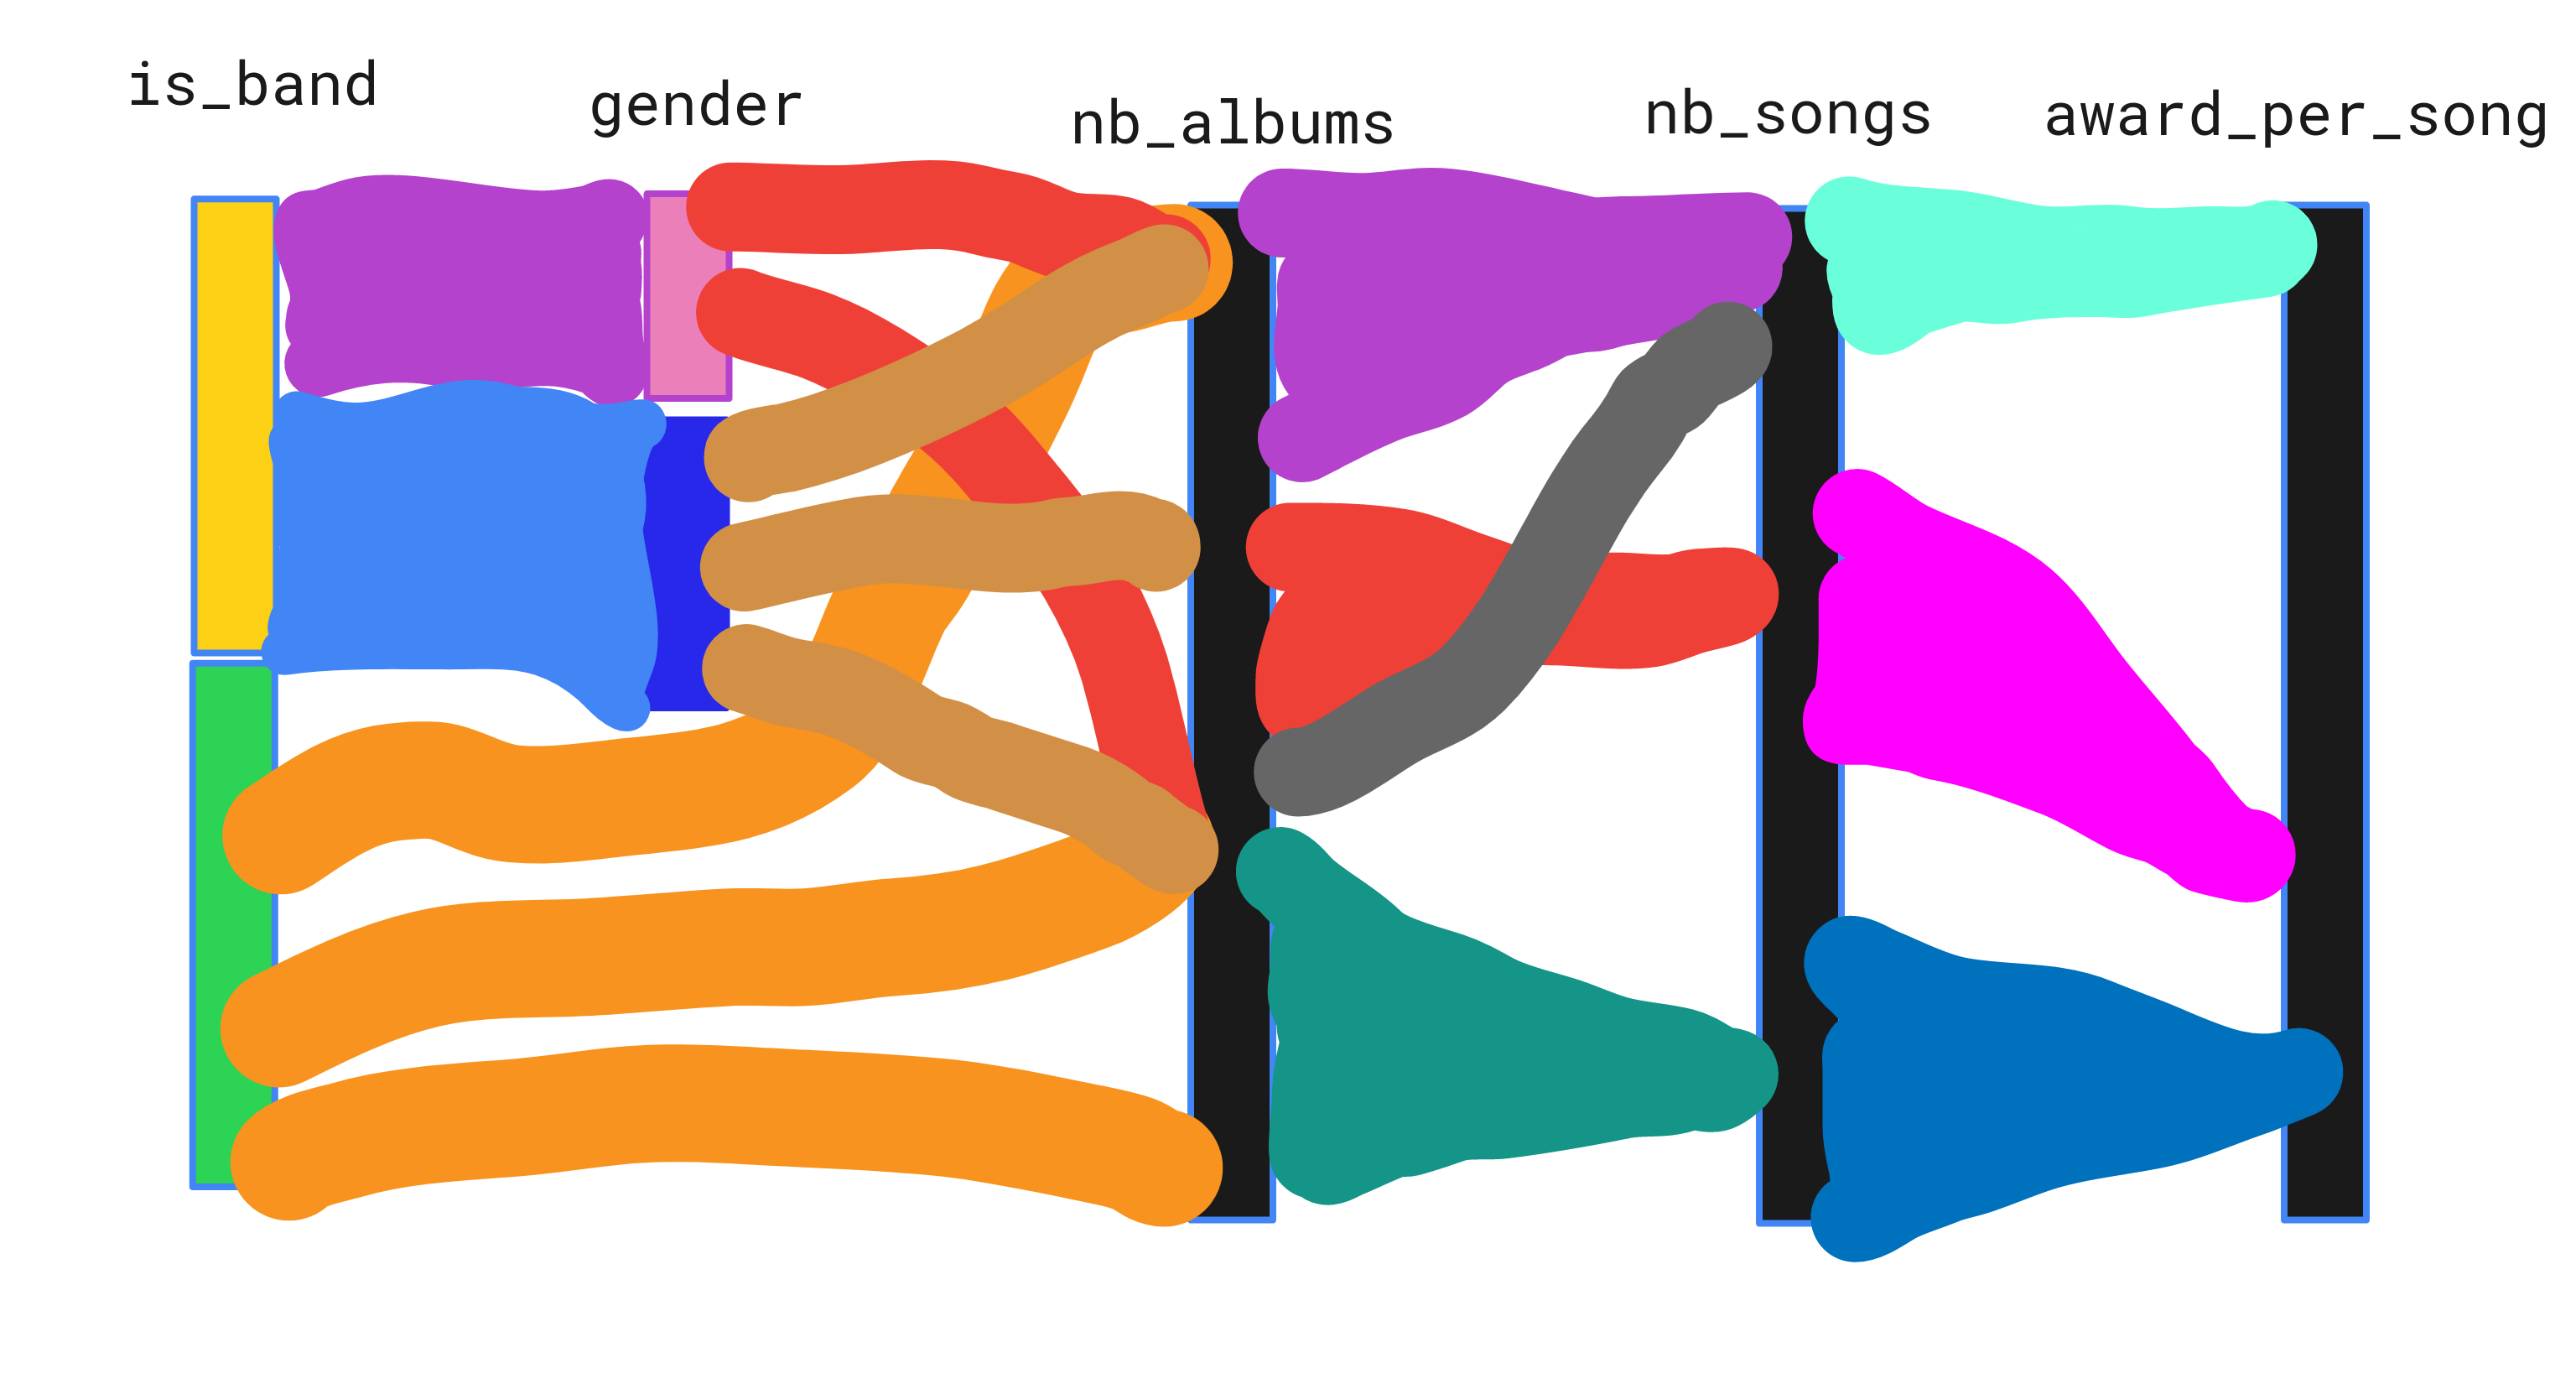
\includegraphics[width=.8\textwidth]{Images/sketch_jl.png}
    \caption{Representation of the Sankey diragram (JL)}
\end{figure}

\section{Protocol UX}
TODO: 
\begin{enumerate}
    \item Write text that will be read (to remove bias in the way I say things)
    \item Test app on some people (minimum 3)
\end{enumerate}

\subsection{Presentation \& training}
\begin{enumerate}
    \item Ask written consent for recording
    \item Tell people why they are here and what we will do
    \item Give the following information:
          \subitem Age
          \subitem Sex
          \subitem Highest level of education reached
    \item Present Sankey diagram and explain what a Sankey diagram is.
    \item Is anything unclear?
\end{enumerate}

\subsection{User test}
\begin{enumerate}
    \item Task 1
          \begin{enumerate}
              \item How many men made 5 albums.
              \item On a scale from 1 to 5 (1 means very easy, 5 means very difficult), how hard was that task?
          \end{enumerate}
    \item Task 2
    \begin{enumerate}
        \item How many rap solo artists are women.
        \item On a scale from 1 to 5 (1 means very easy, 5 means very difficult), how hard was that task?
    \end{enumerate}
    \item Task 3
    \begin{enumerate}
        \item Can you tell how many solo artists made 3 albums? Why/Why not?
        \item On a scale from 1 to 5 (1 means very easy, 5 means very difficult), how hard was that task?
    \end{enumerate}
\end{enumerate}

\subsection{Debriefing}
\begin{enumerate}
    \item What are your three favorite feature?
    \item What is your three least favorite feature?
    \item Would you recommend this application to a friend?
    \item What would you do differently?
\end{enumerate}

\end{document}